\subsubsection*{Valores iniciales:}
\begin{multicols}{2}
	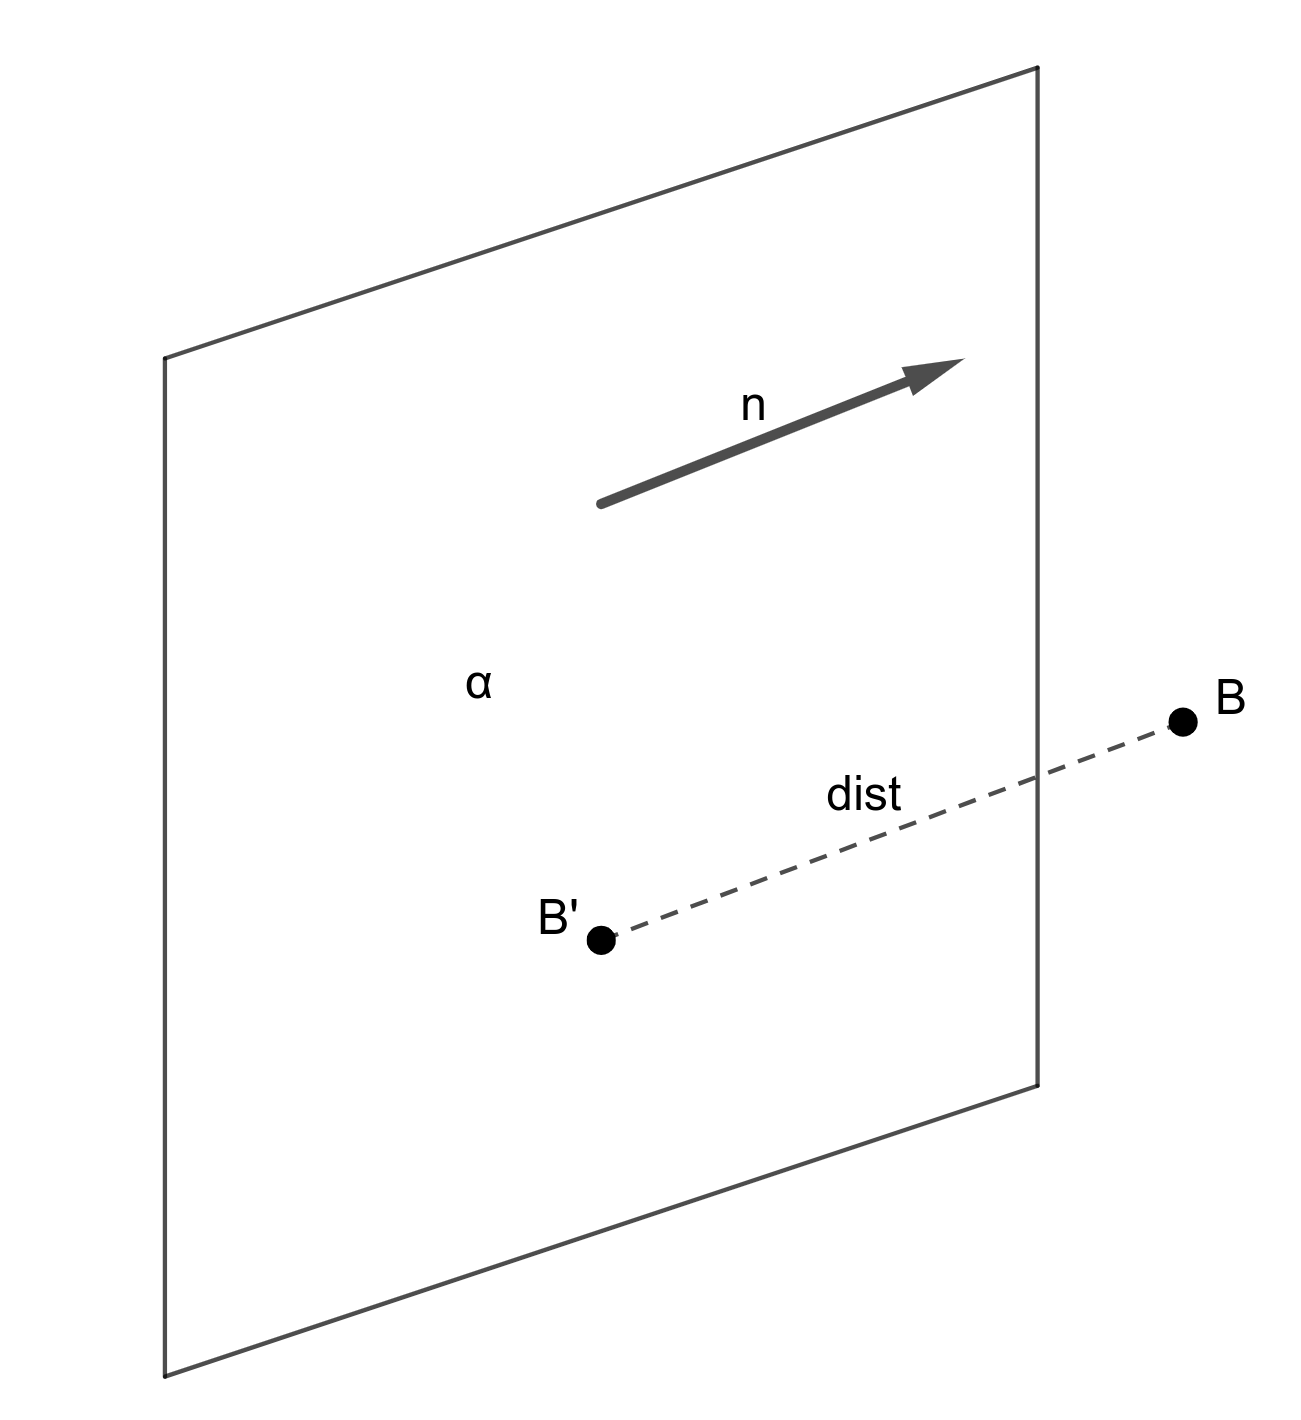
\includegraphics[width=7cm, scale=0.8]{ej-18/18ini.png}

	\noindent Ecuación del plano $\alpha$ dado: \\
	\indent $\alpha) \ \ 3x + 2y -5z = 0$

	\noindent Punto $B$ dado: \\
	\indent $B(2, 1, -1)$

	\noindent Vector $\overrightarrow{OB} = \vec{b}$: \\
	\indent $\vec{b} = (2, 1, -1)$

	\noindent Vector normal del plano: \\
	\indent $\vec{n}=(3, 2, -5)$

	\noindent Ecuaciones paramétricas de una recta ortogonal al plano $\alpha$: \textit{(solo con fines ilustrativos)}

	$r) \ \begin{cases}
			x = 2 + 3t \\
			y = 1 + 2t \\
			z = -1 - 5t
		\end{cases}$
\end{multicols}

\noindent Lo anterior nos presenta la siguiente situación:

\begin{center}
	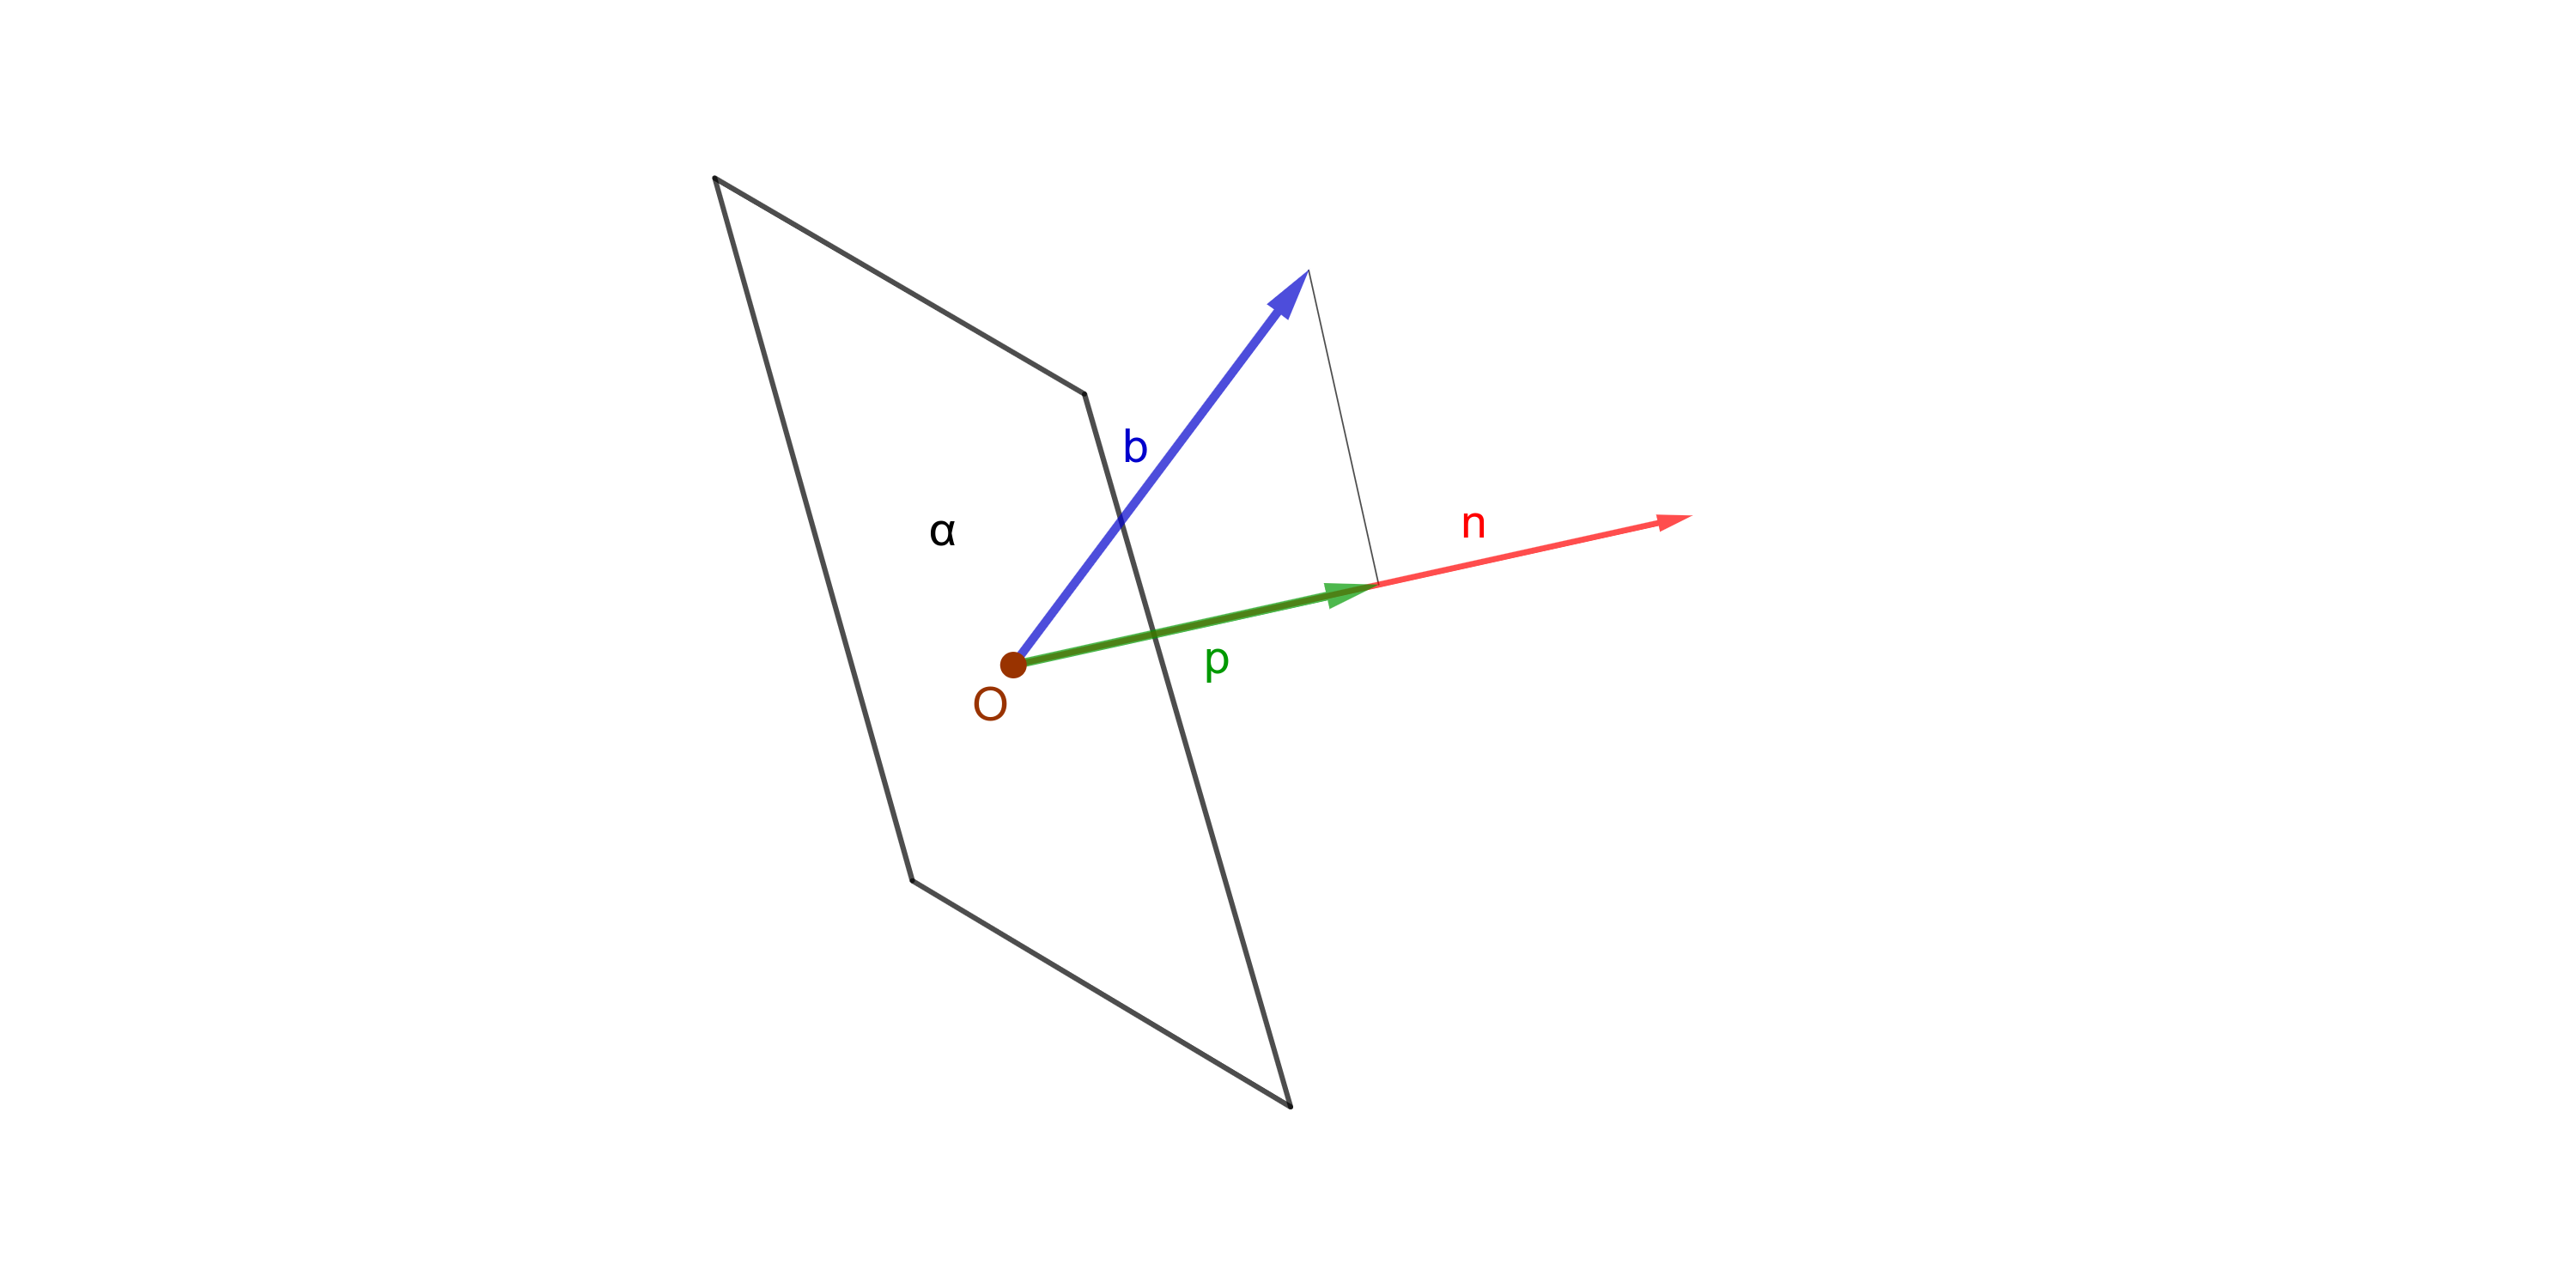
\includegraphics[width=10cm, scale=0.8]{ej-18/18ini2.png}
\end{center}

Ya que el coeficiente $d$ de $\alpha$ es igual a $0$, determinamos que el plano cruza el origen de coordenadas. El vector $\vec{n}$ representa el vector normal $\perp$ a $\alpha$, el vector $\vec{b}$ que representa la distancia $\overline{OB}$, con lo que la distancia del punto $B$ al plano $\alpha$ está determinada por el módulo del vector $\vec{p}$ \textit{(proyección de $\vec{b}$ sobre $\vec{n}$)}, que está dado por:

\begin{center}
	$\boxed{\overrightarrow{Proy_{\vec{n}} \ \vec{b}} = \cfrac{\vec{b} \cdot \vec{n}}{|\vec{n}|^2} \cdot \vec{n} = \vec{p}}$
\end{center}



